%%%%%%%%%%%%%%%%%%%%%%%%%%%%%%%%%%%%%%%%%
% Short Sectioned Assignment LaTeX Template Version 1.0 (5/5/12)
% This template has been downloaded from: http://www.LaTeXTemplates.com
% Original author:  Frits Wenneker (http://www.howtotex.com)
% License: CC BY-NC-SA 3.0 (http://creativecommons.org/licenses/by-nc-sa/3.0/)
%%%%%%%%%%%%%%%%%%%%%%%%%%%%%%%%%%%%%%%%%

%----------------------------------------------------------------------------------------
%	PACKAGES AND OTHER DOCUMENT CONFIGURATIONS
%----------------------------------------------------------------------------------------

\documentclass[paper=a4, fontsize=11pt]{scrartcl} % A4 paper and 11pt font size

% ---- Entrada y salida de texto -----

\usepackage[T1]{fontenc} % Use 8-bit encoding that has 256 glyphs
\usepackage[utf8]{inputenc}
\usepackage{fourier} % Use the Adobe Utopia font for the document - comment this line to return to the LaTeX default

% ---- Idioma --------

\usepackage[spanish, es-tabla]{babel} % Selecciona el español para palabras introducidas automáticamente, p.ej. "septiembre" en la fecha y especifica que se use la palabra Tabla en vez de Cuadro

% ---- Otros paquetes ----

\usepackage{url} % ,href} %para incluir URLs e hipervínculos dentro del texto (aunque hay que instalar href)
\usepackage{amsmath,amsfonts,amsthm} % Math packages
%\usepackage{graphics,graphicx, floatrow} %para incluir imágenes y notas en las imágenes
\usepackage{graphics,graphicx, float} %para incluir imágenes y colocarlas
\usepackage{epstopdf}
\usepackage[gen]{eurosym} %para incluir el símbolo del euro
\usepackage{cite} %para incluir citas del archivo <nombre>.bib
%\graphicspath{/images}

% Para hacer tablas comlejas
%\usepackage{multirow}
%\usepackage{threeparttable}

%\usepackage{sectsty} % Allows customizing section commands
%\allsectionsfont{\centering \normalfont\scshape} % Make all sections centered, the default font and small caps

\usepackage{fancyhdr} % Custom headers and footers
\pagestyle{fancyplain} % Makes all pages in the document conform to the custom headers and footers
\fancyhead{} % No page header - if you want one, create it in the same way as the footers below
\fancyfoot[L]{} % Empty left footer
\fancyfoot[C]{} % Empty center footer
\fancyfoot[R]{\thepage} % Page numbering for right footer
\renewcommand{\headrulewidth}{0pt} % Remove header underlines
\renewcommand{\footrulewidth}{0pt} % Remove footer underlines
\setlength{\headheight}{13.6pt} % Customize the height of the header

\numberwithin{equation}{section} % Number equations within sections (i.e. 1.1, 1.2, 2.1, 2.2 instead of 1, 2, 3, 4)
\numberwithin{figure}{section} % Number figures within sections (i.e. 1.1, 1.2, 2.1, 2.2 instead of 1, 2, 3, 4)
\numberwithin{table}{section} % Number tables within sections (i.e. 1.1, 1.2, 2.1, 2.2 instead of 1, 2, 3, 4)

\setlength\parindent{0pt} % Removes all indentation from paragraphs - comment this line for an assignment with lots of text

\newcommand{\horrule}[1]{\rule{\linewidth}{#1}} % Create horizontal rule command with 1 argument of height


%----------------------------------------------------------------------------------------
%	TÍTULO Y DATOS DEL ALUMNO
%----------------------------------------------------------------------------------------

\title{
\normalfont \normalsize
\textsc{\textbf{Ingeniería de Servidores (2016-2017)} \\ Grado en Ingeniería Informática \\ Universidad de Granada} \\ [25pt] % Your university, school and/or department name(s)
\horrule{0.5pt} \\[0.4cm] % Thin top horizontal rule
\huge Memoria Práctica 5 \\ % The assignment title
\horrule{2pt} \\[0.5cm] % Thick bottom horizontal rule
}

\author{Adrián Morente Gabaldón} % Nombre y apellidos

\date{\normalsize\today} % Incluye la fecha actual

%----------------------------------------------------------------------------------------
% DOCUMENTO
%----------------------------------------------------------------------------------------

\begin{document}

\maketitle % Muestra el Título

\newpage %inserta un salto de página

\tableofcontents % para generar el índice de contenidos

\newpage

\listoffigures

\listoftables

\newpage


\section{[SYSCTL] Al modificar los valores del kernel de este modo, no logramos que persistan después de reiniciar la máquina. ¿Qué archivo hay que editar para que los cambios sean permanentes?}
Como ya se explicó en clase de prácticas, \emph{Sysctl} modifica los parámetros del kernel en tiempo de ejecución, por lo que al reiniciar la máquina se pierden los valores modificados. Si ejecutamos Sysctl a través de línea de comandos sin opciones, se nos despliega una pequeña lista con sus opciones más destacadas, que son las siguientes:
\begin{figure}[H]
	\centering
	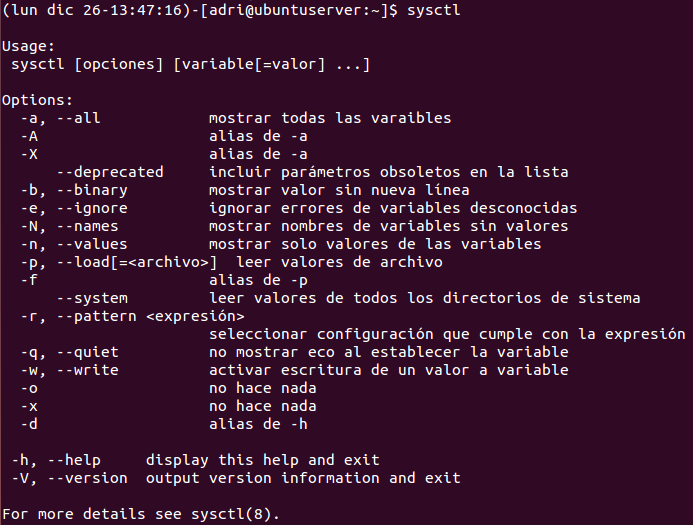
\includegraphics[scale=0.6]{sysctl-h}
	\caption{Opciones más destacadas de sysctl. - Adrián Morente Gabaldón [26/12/2016]}
	\label{figura1}
\end{figure}
Como vemos en la captura de pantalla anterior, el propio sysctl nos redirige a su manual si queremos explorar más opciones u obtener más información. Al principio de este manual, encontramos que todos los parámetros configurables descienden del directorio \emph{/proc/sys}, ordenados en subcarpetas según pertenencia (sistema de archivos, kernel, memoria virtual, etc), y cada uno de ellos se encuentra en formato de archivo en texto plano, conteniendo tan solo el valor del parámetro en cuestión. Veamos un ejemplo de los parámetros pertenecientes al módulo de memoria virtual:
\begin{figure}[H]
	\centering
	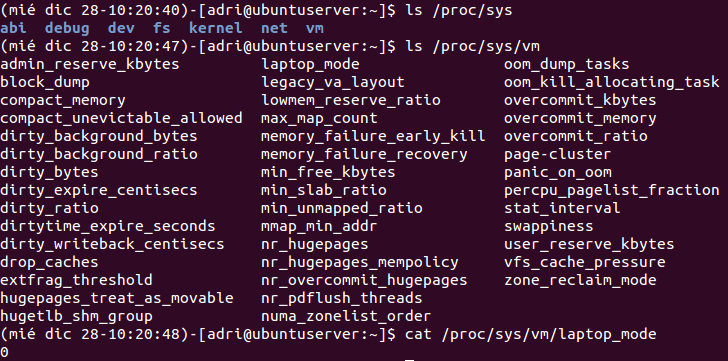
\includegraphics[scale=0.7]{proc-sys}
	\caption{Contenido del directorio /proc/sys, sus subdirectorios y ejemplo de uno de sus parámetros. - Adrián Morente Gabaldón [28/12/2016]}
	\label{figura3}
\end{figure}
Para que los cambios persistan tras reiniciar la máquina, debemos aplicar la modificación a cada uno de los ficheros de parámetros. Sin embargo, por temas de seguridad, es mejor utilizar esta herramienta con algunas de sus múltiples opciones en lugar de acceder y modificar directamente dichos ficheros (ya que podemos ``tocar donde no debemos''). 


\section{¿Con qué opción se muestran todos los parámetros modificables en tiempo de ejecución? Elija dos parámetros y explique, en dos líneas, qué función tienen.}
Si leemos el manual de sysctl en la terminal, vemos rápidamente que la opción para consultar todas las variables modificables en ejecución es \emph{-a}:
\begin{figure}[H]
	\centering
	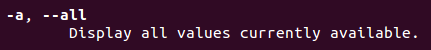
\includegraphics[scale=0.7]{sysctl-a}
	\caption{Opción de Sysctl para consultar los parámetros modificables en ejecución. - Adrián Morente Gabaldón [26/12/2016]}
	\label{figura2}
\end{figure}
Si ejecutamos \textbf{sysctl -a} obtenemos una extensa lista con todas las variables configurables. Exactamente, tantas como ficheros había en los subdirectorios de \emph{/proc/sys} vistos en el ejercicio anterior, lógicamente.

\section{[Windows Server] a) Realice una copia de seguridad del registro y restáurela, ilustre el proceso con capturas. b) Abra una ventana mostrando el editor del registro.}
Para empezar, seguiremos las instrucciones dictadas por el guión de prácticas, comenzando por ejecutar \emph{regedit} desde la línea de comandos de Windows Server. A continuación, nos encontraremos con esta ventana:
\begin{figure}[H]
	\centering
	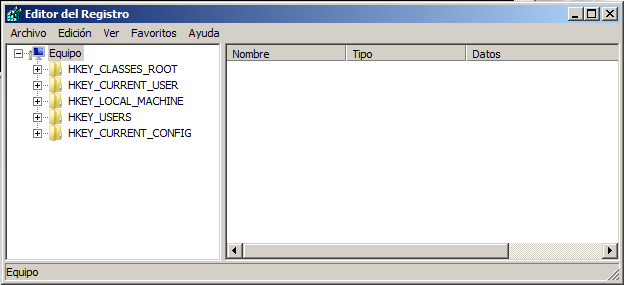
\includegraphics[scale=0.7]{regedit}
	\caption{Ventana principal del Editor del Registro en Windows Server. - Adrián Morente Gabaldón [26/12/2016]}
	\label{figura4}
\end{figure}


\section{Enumere qué elementos se pueden configurar en Apache y en IIS para que Moodle funcione mejor.}


\section{Ajuste la compresión en el servidor y analice su comportamiento usando varios valores para el tamaño de archivo a partir del cual comprimir. Para comprobar que está comprimiendo puede usar el navegador o comandos como curl (see url) o lynx. Muestre capturas de pantalla de todo el proceso.}


\section{a) Usted parte de un SO con ciertos parámetros definidos en la instalación (Práctica 1), ya sabe instalar servicios (Práctica 2) y cómo monitorizarlos (Práctica 3) cuando los somete a cargas (Práctica 4). Al igual que ha visto cómo se puede mejorar un servidor web (Práctica 5 Sección 3.1), elija un servicio (el que usted quiera) y modifique un parámetro para mejorar su comportamiento. b) Monitorice el servicio antes y después de la modificación del parámetro aplicando cargas al sistema (antes y después) mostrando los resultados de la monitorización.}

\section{PREGUNTAS OPCIONALES}
	\subsection{Realice lo mismo que en la cuestión 6 pero para otro servicio.}




\bibliography{citas}
\bibliographystyle{plain}
\end{document}
